%% The first command in your LaTeX source must be the \documentclass command.
%%
%% Options:
%% twocolumn : Two column layout.
%% hf: enable header and footer.
\documentclass[
    hf
]{ceurart}
\usepackage[top=2.5cm, bottom=2.5cm, left=2.5cm, right=2.5cm]{geometry}

%%
%% One can fix some overfulls
\sloppy

%%
%% Minted listings support 
%% Need pygment <http://pygments.org/> <http://pypi.python.org/pypi/Pygments>
\usepackage[frozencache,cachedir=./_minted-bdi]{minted}
%% auto break lines
\setminted{breaklines=true}
\usepackage[utf8]{inputenc}	% allow utf-8 input
\usepackage{placeins} % for FloatBarrier
\usepackage{adjustbox} % to squeeze tables to textwidth
\usepackage{subcaption}

\usepackage[backend=biber]{biblatex}
\addbibresource{bibliography.bib}

%%
%% end of the preamble, start of the body of the document source.
\begin{document}

%%
%% Rights management information.
%% CC-BY is default license.
\copyrightyear{2024}
\copyrightclause{Copyright for this paper by its authors.
    Use permitted under Creative Commons License Attribution 4.0
    International (CC BY 4.0).}

%%
%% This command is for the conference information
% \conference{CHR 2022: Computational Humanities Research Conference, December 12 -- 14,
%     2022, Antwerp, Belgium}
\conference{CHR 2024: Computational Humanities Research Conference, December 4--6, 2024. Aarhus, Denmark }
%%
%% The "title" command
\title{Bootstrap Distance Imposters: High precision authorship verification with improved interpretability}
\shorttitle{Bootstrap Distance Imposters}

\tnotemark[1]
\tnotetext[1]{I am grateful to various members of the Computational Stylistics Group
    \url{https://computationalstylistics.github.io/} for their ideas and support. Particular thanks
    are due to Mike Kestemont for a kind but careful review of the initial draft; subsequent errors
    are my own. I thank the anonymous CHR reviewers for their thoughtful comments, some of
    which could not be implemented in time for proceedings but offer exciting potential for further
    work.}

%%
%% The "author" command and its associated commands are used to define
%% the authors and their affiliations.
\author[1]{Ben Nagy}[%
    orcid=0000-0002-5214-7595,
    url=https://github.com/bnagy/bdi-paper,
    email=benjamin.nagy@ijp.pan.pl,
]
\address[1]{Institute of Polish Language, Polish Academy of Sciences (IJP PAN)\\
    al. Mickiewicza 31\\
    Kraków, Poland}
%%
%% The abstract is a short summary of the work to be presented in the
%% article.
\begin{abstract}
    This paper describes an update to the open-source Python implementation of the General Imposters
    method of authorship verification by Mike Kestemont et al. The new algorithm, called Bootstrap
    Distance Imposters (henceforth BDI), incorporates a key improvement introduced by Potha and
    Stamatatos, as well as introducing a novel method of bootstrapping that has several attractive
    properties when compared to the reference algorithm. Initially, we supply an updated version of
    the Kestemont et al. code (for Python 3.x) which incorporates the same basic improvements. Next,
    the two approaches are benchmarked using the problems from the multi-lingual PAN 2014 author
    identification task, as well as the more recent PAN 2021 task. Additionally, the
    interpretability advantages of BDI are showcased via real-world verification studies. When
    operating as a summary verifier, BDI tends to be more conservative in its positive attributions,
    particularly when applied to difficult problem sets like the PAN2014 \textit{en\_novels}. In
    terms of raw performance, the BDI verifier outperforms all PAN2014 entrants and appears slightly
    stronger than the improved Kestemont GI according to the PAN metrics for both the 2014 and 2021
    problems, while also offering superior interpretability.
\end{abstract}

%% Keywords. The author(s) should pick words that accurately describe
%% the work being presented. Separate the keywords with commas.
\begin{keywords}
    authorship verification \sep
    stylometry \sep
    bootstrapping
\end{keywords}

%%
%% This command processes the author and affiliation and title
%% information and builds the first part of the formatted document.
\maketitle

\section{Introduction}

A common task in the field of stylometry is to attempt to resolve questions of authorship. In
``authorship verification'' the basic question is ``how likely is it that a given document is by a
specified author?''. Since the answers to these questions can have important repercussions, whether
legal, literary, or social, it is important that the methods employed by practitioners be reliable;
but in order for the results to be believed they should also be transparent and interpretable. The
General Imposters method (henceforth GI), originally formulated by Koppel and Winter in
\cite{koppel_gi}, has become one of the standard methods in stylometry for authorship verification.
After strong performances in the PAN 2013 and 2014 competitions, it was implemented and used by M.
Kestemont et al. in an influential study \cite{kestemont_caesar}, improved by Potha and Stamatatos
in 2017 \cite{potha_improved_gi}, and is now available in the well-known R package \emph{stylo}
\cite{stylo}.

In this paper I describe an update to the open-source Python implementation by Kestemont et al.
\cite{kestemont_ruzicka} called Bootstrap Distance Imposters (henceforth BDI) which incorporates
several of the improvements proposed since the last release, as well as introducing a novel method
of bootstrapping that has several attractive properties when compared to the reference algorithm.
The two approaches are benchmarked using the problems from the PAN 2014 author identification task
\cite{pan_2014}, and some additional properties are showcased via real-world case studies.

\section{Motivation and Design}

\begin{figure*}
    \centering
    \begin{subfigure}{.5\textwidth}
        \centering
        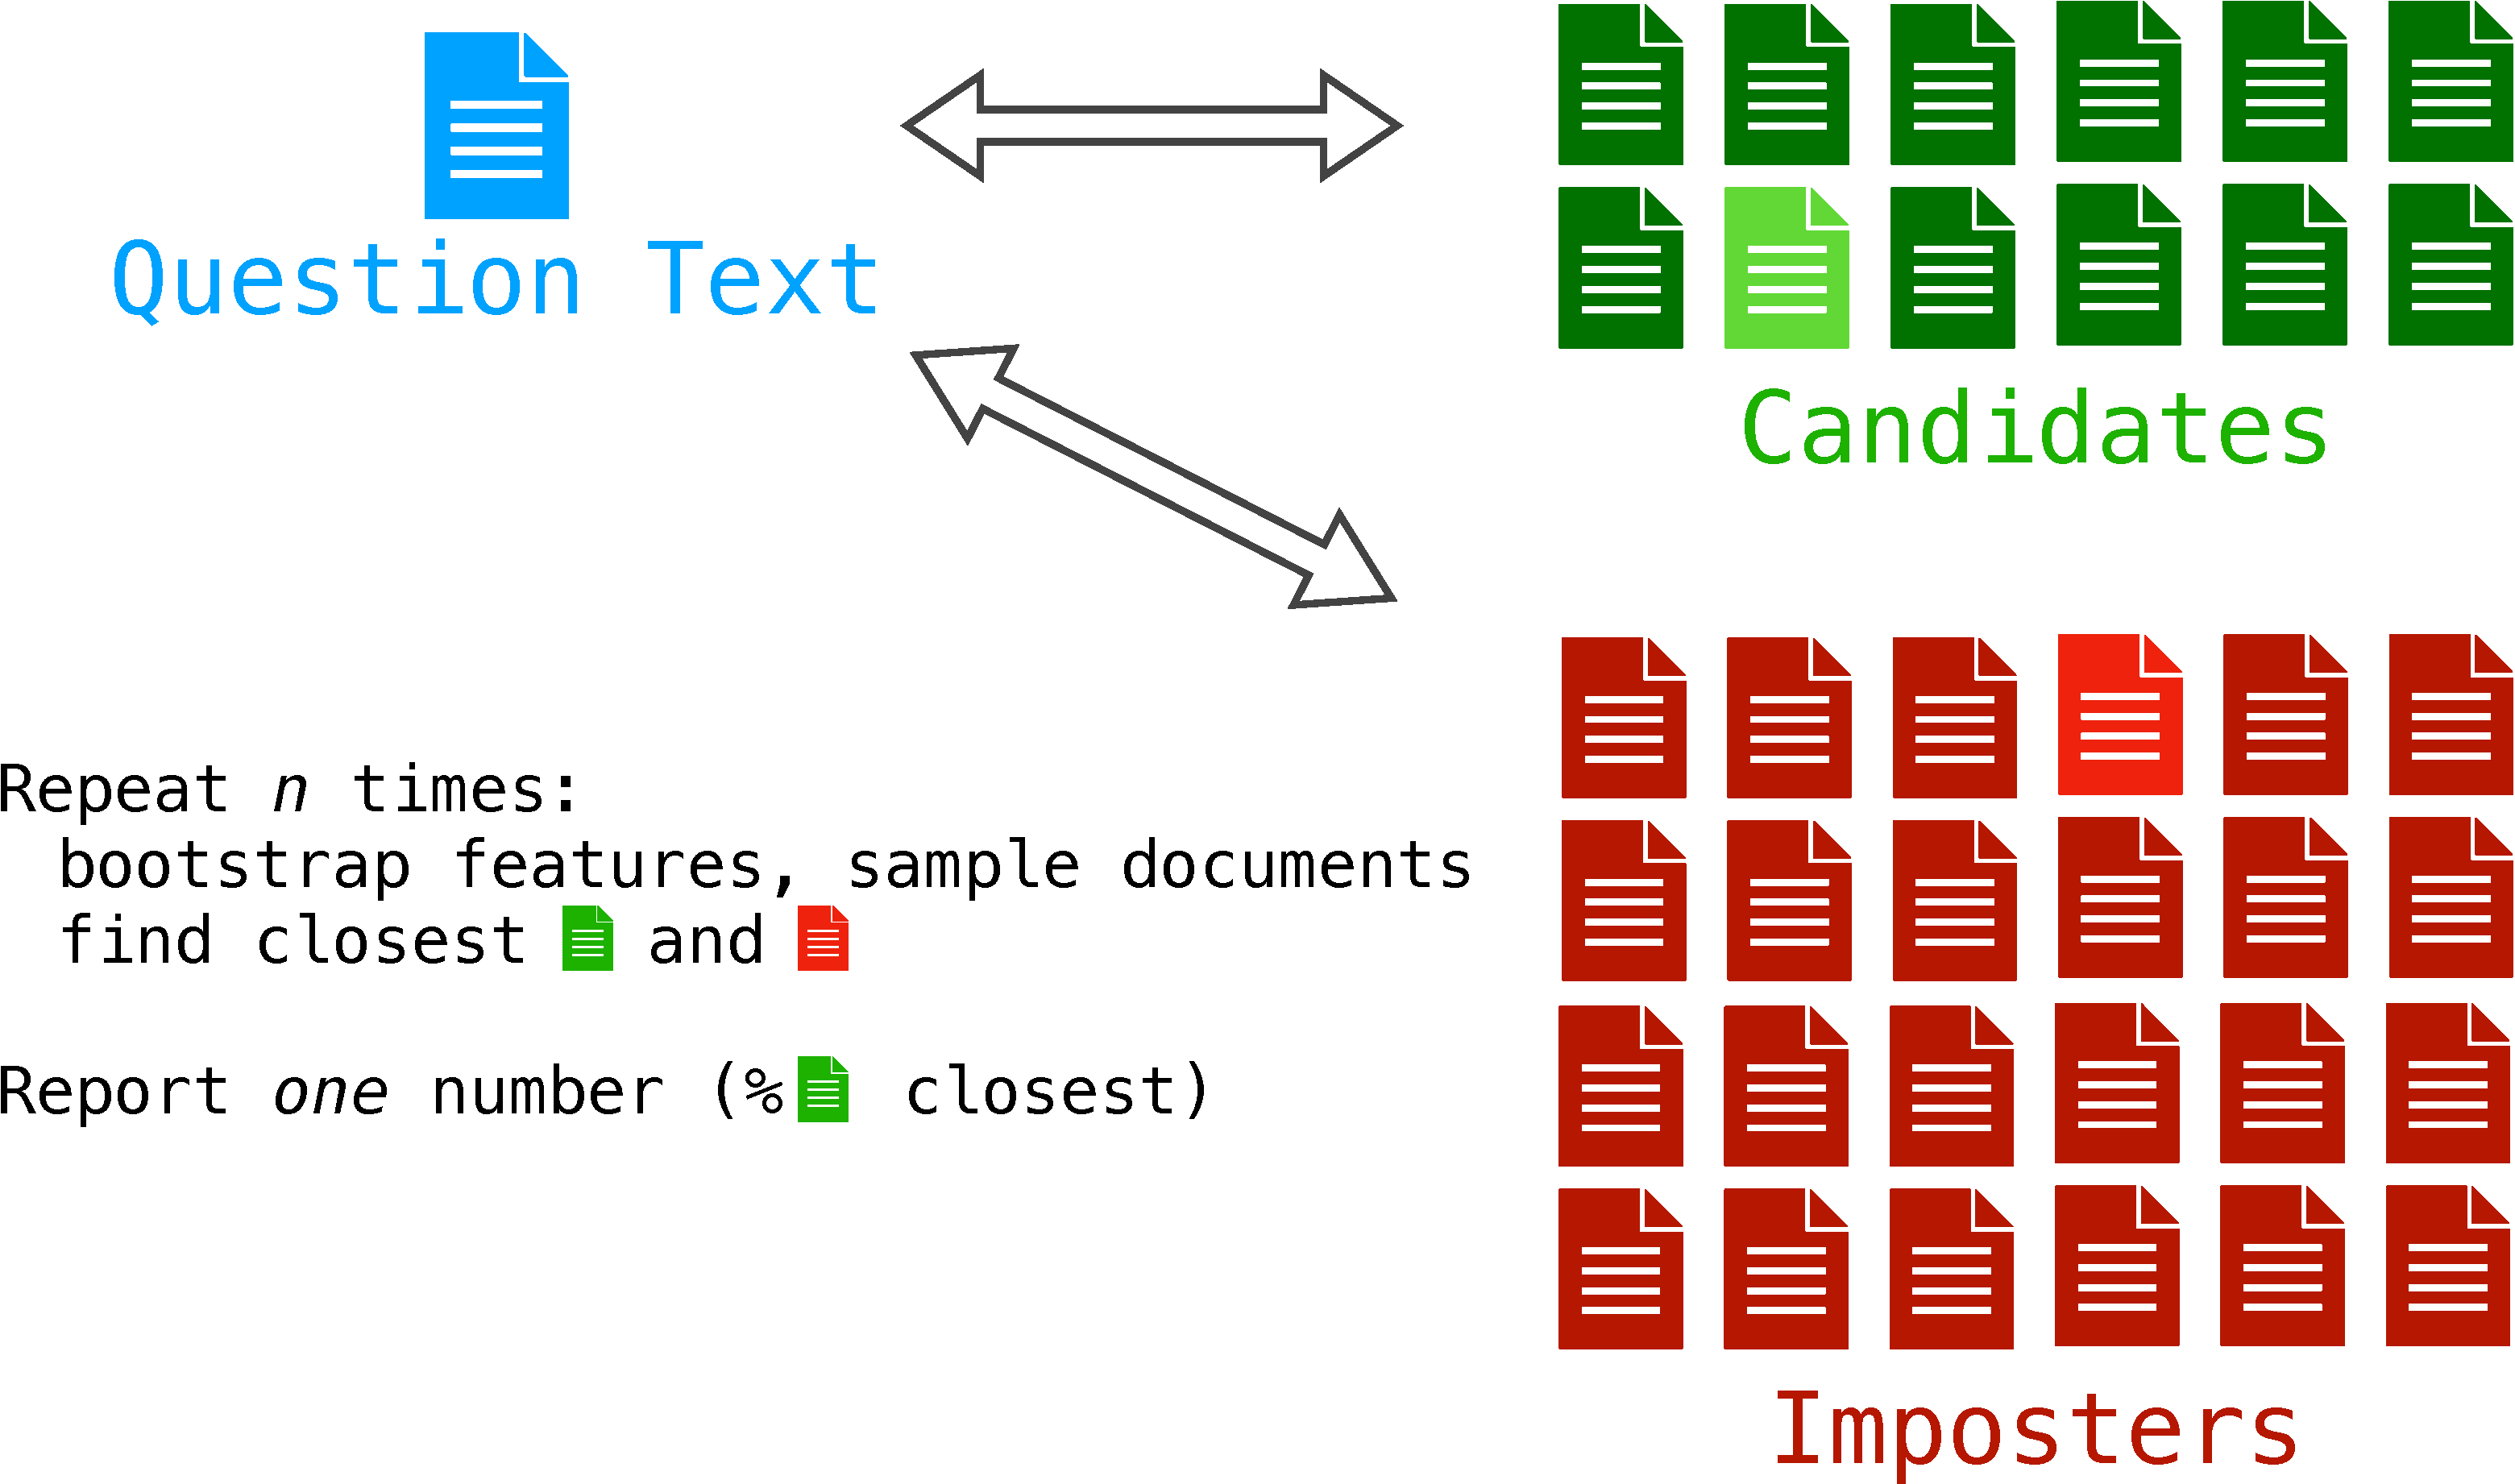
\includegraphics[width=0.93\linewidth]{images/bdi_graphic_gi-crop.pdf}
        \caption*{Standard General Imposters}
    \end{subfigure}% <-- LOAD BEARING PERCENT SIGN
    \begin{subfigure}{.5\textwidth}
        \centering
        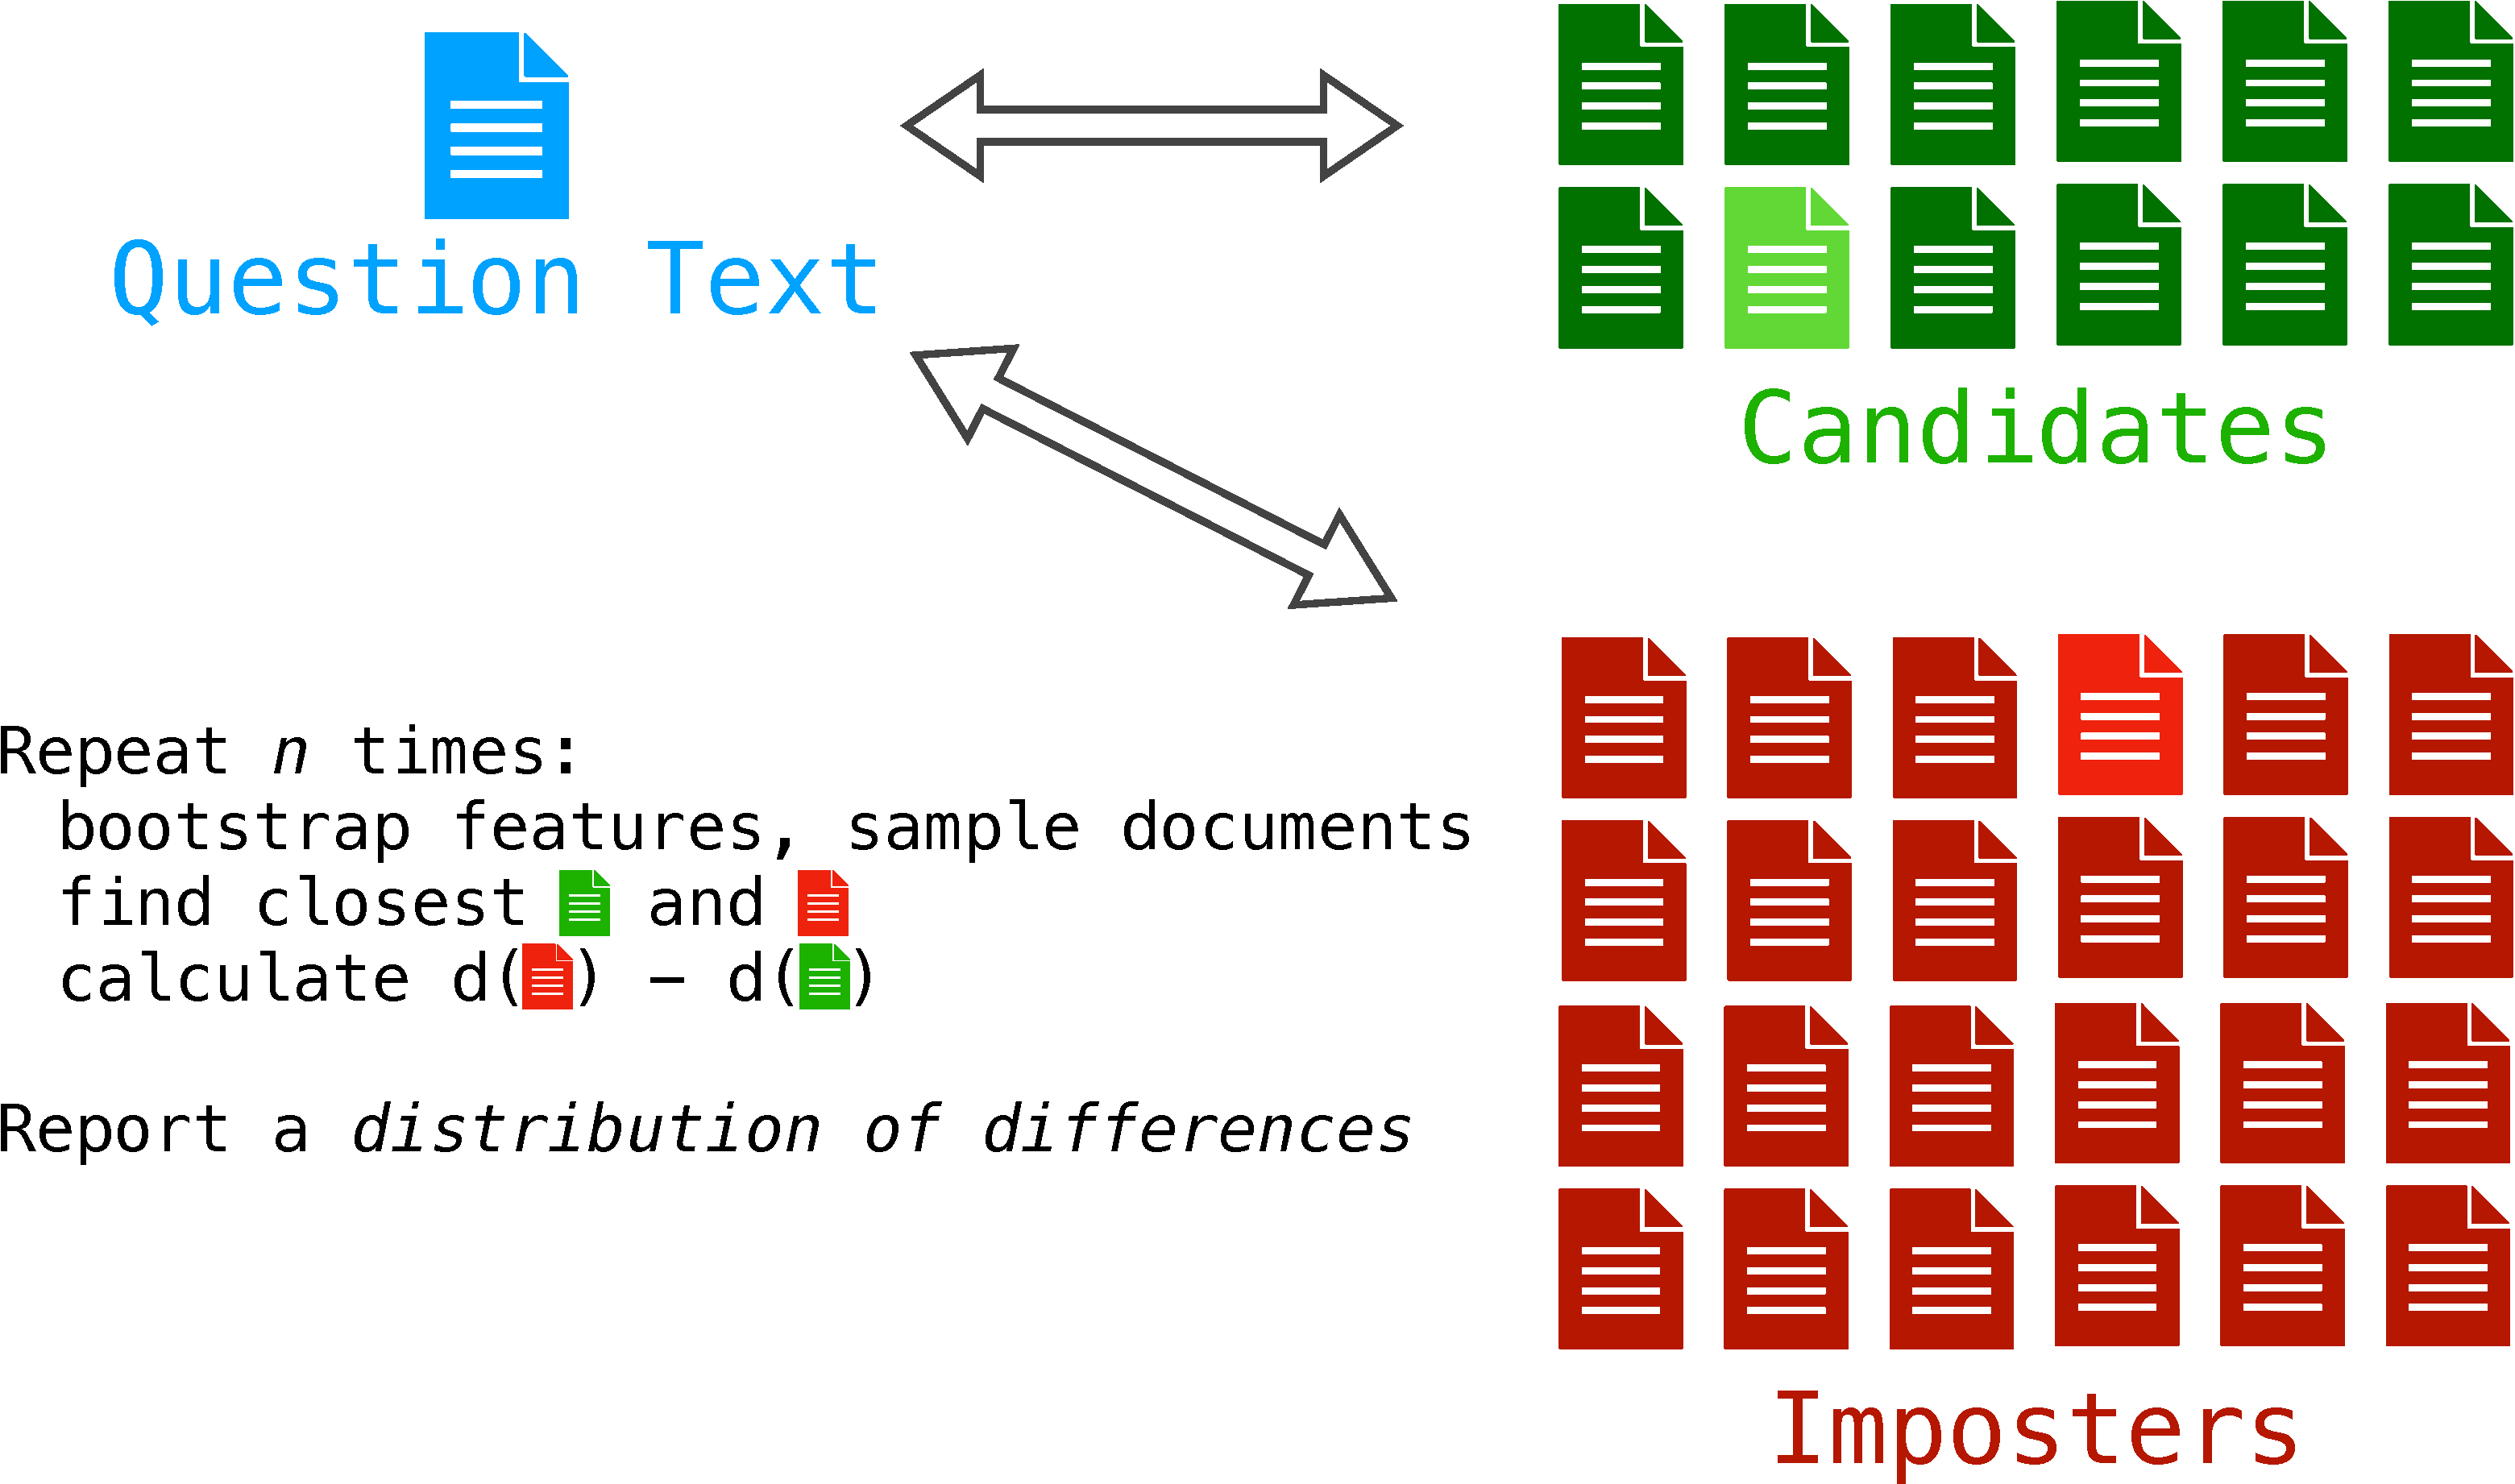
\includegraphics[width=0.93\linewidth]{images/bdi_graphic_bdi-crop.pdf}
        \caption*{Bootstrap Distance Imposters}
    \end{subfigure}%
    \caption{A simplified comparison of the operation of `standard' General Imposters and
        Bootstrap Distance Imposters.}
    \label{fig:gibdi}
\end{figure*}

The Imposters method of authorship verification examines a \emph{question text} in order to
determine whether the text was written by a \emph{candidate author}. To do this, it performs
bootstrap comparisons of the question text to candidate texts and several (perhaps very many)
\emph{imposter texts} which should ideally be chosen to be similar in genre, topic and register. If
the question text is markedly more similar to the candidate author's `style' than to any of the
imposters then we infer, with some level of statistical likelihood, that it was authored by the
candidate. The method of Imposters can be used with any features that reflect style, although it is
most commonly applied to distances between character $n$-gram or word frequency vectors.

Note that while I speak of `statistical likelihood' I am carefully avoiding the words `probability'
and `confidence'. The GI method is, in machine learning terms, an ensemble classifier. These
classifiers regularise well, but while they produce a real-valued output, it is problematic to
interpret this number as a probability. Many factors can make the verification results less
reliable---the lengths of the texts, the language in which they are written, the closeness of the
imposter texts (dissimilar texts make a positive attribution less convincing), and the amount of
available data (a lack of comparison data risks bias). Verification problems in the real world are
seldom under ideal conditions, and there is no magical formula by which the uncertainties imposed by
the problem setting can be convincingly rendered as a forensic probability. Never the less, the
Imposters method has a well deserved reputation for robust, understandable results, even in the face
of severe limitations (for example in the length of samples or the availability of suitable
imposters).

Figure \ref{fig:gibdi} attempts an intuitive explanation of the basic operation of standard GI and
the key modification used in BDI. The output of the Kestemont GI classifier is a percentage of
binarized `votes' (the number of times a candidate text was closer than an imposter). In contrast,
the raw output from the BDI algorithm is a bootstrapped distribution of differences. At each step,
the distance (with a bootstrapped feature set) between the candidates and the imposters is recorded,
using any vector distance measure $d: \mathbb{R}^n \times \mathbb{R}^n \rightarrow \mathbb{R}$. If
the candidates are further, the difference between the distances is negative, if closer it is
positive. If these individual distances follow a Gaussian distribution (which is a reasonable prior
expectation) then their difference is also Gaussian. Expressing the results this way has some
advantages. The first is that we can differentiate a negative result (not the candidate) as either
`none of the above' or `more like an imposter' (the true author is in the imposters set). A `none of
the above' result would have a statistically expected distance of zero (equally unlike the candidate
and the imposters), and so we would see a distribution centred around 0.%
%
\footnote{ Note carefully that this is a one-way implication---a true author
    that is neither the candidate nor one of the imposters should have a
    distance distribution centred around zero, but not all such distributions
    guarantee that the true author is not among the imposters.}
%
On the other hand, `more like an imposter' results show distributions centred around a negative
value (examples of this can be seen in Section \ref{sec:showcase} below). The other advantage is
that for strong positives, we have additional data about the match. Distributions centred around
larger positive numbers are better matches, but distributions with high variance show more feature
dependence (since the strength of the match varies greatly depending on the bootstrap feature sets).
In summary, positive matches (with most or all of the probability mass above zero) can be much more
meaningfully compared.

It is worth noting here that the overall best performing method at PAN 2014 by Khonji and Iraqi
\cite{khonji_iraqi} also modified the classic GI algorithm to utilize the distance between vectors
(in that case the relative distance of the test vector to candidates vs imposters was considered as
part of the decision function for a `standard' voting-based classifier), so this paper is not the
first to recognise the value of this additional information.

\subsection{Binary Classification}

Based on the BDI algorithm, which outputs a distribution, it is obviously useful to have a summary
statistic that can be interpreted as evidence for authorship verification tasks. For this paper I
used a simple approach that considers the amount of probability mass that lies above 0. If every
test is closer to a candidate than an imposter then the result will be 1, if every test is more like
an imposter, it will be 0, etc. This is implemented simply as the inverse percentile of (a distance
of) 0. Thus armed with a method that outputs a `probability-like' result in $[0,1]$, I wrapped the
code in a classifier that follows \texttt{scikit-learn} \cite{scikit-learn} conventions like
\texttt{fit()} and \texttt{predict\_proba()} and evaluated the BDI classifier directly against the
updated Kestemont GI \texttt{Order2Verifier} using the PAN shared tasks from 2014 and 2021. This
provided a convenient benchmark, and also an opportunity to compare the results against a number of
other verification approaches.

\subsection{Score Shifting}

The C@1 metric introduced in PAN 2014 rewards (or at least penalises less harshly) classifiers that
choose not to answer some problems. This leads naturally to algorithms that use the training data to
define classifier output ranges that will be assigned to 0.5 (indicating an unanswered problem). In
the case of classic GI, this means that classifier scores (vote percentages) within certain ranges
will be rectified to precisely 0.5, while positive and negative classifications are shifted to the
ranges above and below that value. This (hopefully) improves the C@1 score as compared to basic
accuracy. In the PAN 2020--21 competitions, a similar measure was used called F$_{0.5u}$ (introduced
in \cite{bevendorff-etal-2019-generalizing}).

The score shifting method implemented in Kestemont GI attempts to produce something more like a
probability by linearly scaling the output values. The code defines an upper and lower bound for the
unanswered region, \texttt{p1} and \texttt{p2} The scaling code (in Python) looks like this:

\begin{minted}{python}
    for score in list(scores):
        if score <= p1:
            new_scores.append(rescale(score, min(scores), max(scores), 0.0, p1))
        elif score >= p2:
            new_scores.append(rescale(score, min(scores), max(scores), p2, 1.0))
        else:
            new_scores.append(0.5)
\end{minted}

Scores below \texttt{p1} are scaled to $[0,\texttt{p1})$, scores above \texttt{p2} are scaled to
$(\texttt{p2},1]$, and the rest are coerced to 0.5. There is an issue with this scaling algorithm,
however. Since \texttt{p1} and \texttt{p2} are chosen by grid search to maximise the PAN score, the
score shifter sometimes fits values for \texttt{p2} that are well below 0.5. This can lead to
decisions that are defined as positive (since they are above \texttt{p2}) being scaled to below 0.5,
where they are evaluated by the scoring metrics as a negative result (and scored as such). In the
updated code, I modified the shifting code to scale more simply to $[0,0.5)$ (negative), 0.5
(unanswered), and $(0.5,1]$ (positive). This does not retain the global distributional properties of
the original results (as implemented in \cite{kestemont_caesar}).

\begin{minted}{python}
    for score in scores: 
        if score <= p1: 
            new_scores.append( rescale(score, orig_min=0, orig_max=p1, new_min=0.0, new_max=0.499) ) 
        elif score >= p2: 
            new_scores.append( rescale(score, orig_min=p2, orig_max=1, new_min=0.501, new_max=1.0) )
        else: 
            new_scores.append(0.5)
\end{minted}

Based on the evaluation problems, the BDI algorithm is not as sensitive to this score shifting,
deriving only a modest benefit from fitting. The fitting process raises natural questions about the
representativeness of the training data, and also causes some problems in domains that suffer from
limited data availability (where it can be hard to sacrifice data for training). In these
circumstances, BDI works well with manual score shifting, allowing the user to choose a confidence
level empirically.

\subsection{Changes to Kestemont GI}

As is the nature of software, the code in the repository documenting the GI algorithm and for the
related work on the Caesarian corpus no longer ran. I reworked the code slightly, and made the
following small changes, which are available in my own repository \cite{nagy_ruzicka}.

\begin{itemize}
    \item Update the code to work with Python 3 (these minimal changes have been incorporated into
          the original repository based on a PR);
    \item Implement a fast `nini' metric (fuzzy Jaccard similarity) as described in \cite{nini_aa};
    \item Implement the Potha \& Stamatatos `ranking' improvement for the consensus score%
          %
          \footnote{ Instead of a strict 1 (candidate closest) or 0 (candidate not closest), Potha
              \& Stamatatos proposed a score improvement based on the ordinal rank of the closest
              candidate, so if a candidate was the second-closest, the score for that iteration
              would be $\frac{1}{2}$. The same paper proposed a distance-based culling method to
              select more relevant imposters, but this was not implemented because of poor Big-O
              complexity.}
          %
          described in \cite{potha_improved_gi};
    \item Remove most non-core code;
    \item Modify the score-shifting algorithm, as described above.
\end{itemize}

\section{Evaluation}

\begin{table}
    \caption{Global micro-average results. PAN21 and PAN14 refer to the overall evaluation metrics
    used in each competition. PAN14-U(nranked) is the overall PAN 2014 score for each classifier
    when run without the ranking improvement.}
    \label{tab:micro}
    \begin{adjustbox}{max width=\textwidth}
        \begin{tabular}{lllrrrrrrrrr}
            \toprule
                                                      &                                     &         & AUC            & C@1            & F_{0.5u}        & F_1            & Brier          & Prec           & PAN21          & PAN14          & PAN14-U        \\
            Verifier                                  & Vectorizer                          & Shifter &                &                &                &                &                &                &                &                &                \\
            \midrule
            \multirow[c]{4}{*}{BDI, Cosine }          & \multirow[c]{2}{*}{ 2,3,4,5-grams } & fitted  & 0.718          & 0.696          & 0.686          & 0.616          & 0.731          & 0.849          & 0.689          & 0.500          & 0.465          \\
                                                      &                                     & manual  & 0.719          & 0.654          & 0.541          & 0.482          & 0.717          & 0.944          & 0.623          & 0.470          & 0.426          \\
                                                      & \multirow[c]{2}{*}{ 2,3,4-grams }   & fitted  & 0.729          & 0.691          & 0.678          & 0.611          & 0.735          & 0.821          & 0.689          & 0.504          & 0.463          \\
                                                      &                                     & manual  & 0.727          & 0.655          & 0.525          & 0.478          & 0.724          & 0.952          & 0.622          & 0.476          & 0.424          \\
            \multirow[c]{4}{*}{BDI, Minmax }          & \multirow[c]{2}{*}{ 2,3,4,5-grams } & fitted  & 0.731          & 0.703          & 0.694          & 0.625          & 0.738          & 0.852          & 0.698          & 0.514          & 0.460          \\
                                                      &                                     & manual  & 0.732          & 0.665          & 0.555          & 0.493          & 0.722          & 0.936          & 0.633          & 0.487          & 0.414          \\
                                                      & \multirow[c]{2}{*}{ 2,3,4-grams }   & fitted  & \textbf{0.737} & \textbf{0.706} & \textbf{0.707} & 0.632          & 0.739          & 0.846          & \textbf{0.704} & \textbf{0.520} & 0.458          \\
                                                      &                                     & manual  & 0.731          & 0.663          & 0.551          & 0.500          & 0.728          & \textbf{0.956} & 0.634          & 0.485          & 0.412          \\
            \multirow[c]{4}{*}{Kestemont GI, Cosine } & \multirow[c]{2}{*}{ 2,3,4,5-grams } & fitted  & 0.723          & 0.673          & 0.660          & 0.650          & 0.784          & 0.788          & 0.698          & 0.487          & 0.457          \\
                                                      &                                     & manual  & 0.689          & 0.548          & 0.500          & 0.699          & 0.783          & 0.918          & 0.644          & 0.378          & 0.428          \\
                                                      & \multirow[c]{2}{*}{ 2,3,4-grams }   & fitted  & 0.715          & 0.664          & 0.645          & 0.642          & 0.780          & 0.778          & 0.689          & 0.475          & 0.456          \\
                                                      &                                     & manual  & 0.693          & 0.548          & 0.498          & 0.714          & 0.784          & 0.926          & 0.647          & 0.380          & 0.414          \\
            \multirow[c]{4}{*}{Kestemont GI, Minmax } & \multirow[c]{2}{*}{ 2,3,4,5-grams } & fitted  & 0.723          & 0.674          & 0.662          & 0.634          & 0.782          & 0.835          & 0.695          & 0.487          & 0.470          \\
                                                      &                                     & manual  & 0.700          & 0.568          & 0.513          & 0.700          & 0.785          & 0.912          & 0.653          & 0.398          & 0.444          \\
                                                      & \multirow[c]{2}{*}{ 2,3,4-grams }   & fitted  & 0.721          & 0.666          & 0.652          & 0.649          & 0.784          & 0.809          & 0.694          & 0.480          & \textbf{0.479} \\
                                                      &                                     & manual  & 0.703          & 0.562          & 0.515          & \textbf{0.719} & \textbf{0.788} & 0.929          & 0.658          & 0.395          & 0.435          \\
            \bottomrule
        \end{tabular}
    \end{adjustbox}
\end{table}

\begin{table}
    \caption{BDI 2,3,4,5-grams, Minmax, Manual Shifter, U$_{count}$ is the number of unanswered
    problems. Summary scores between U$_{low}$ and U$_{high}$ are left unanswered (changed to
    0.5).}
    \label{tab:bdi}
    % \par\medskip
    \raggedright
    \begin{adjustbox}{max width=\textwidth}

        \begin{tabular}{lrrrrrrrrrrrr}
            \toprule
            Corpus & Tests & U_{count} & U_{low} & U_{hi} & Prec & AUC & C@1 & F_{0.5u} & F_1 & Brier & PAN21 & PAN14 \\
            \midrule
            du\_essays & 96 & 20 & 0.110 & 0.890 & 0.951 & 0.952 & 0.919 & 0.871 & 0.963 & 0.916 & 0.924 & 0.875 \\
            du\_reviews & 50 & 10 & 0.110 & 0.890 & 0.667 & 0.594 & 0.552 & 0.250 & 0.190 & 0.630 & 0.443 & 0.328 \\
            en\_essays & 200 & 27 & 0.110 & 0.890 & 1.000 & 0.638 & 0.568 & 0.231 & 0.141 & 0.634 & 0.442 & 0.362 \\
            en\_novels & 200 & 28 & 0.110 & 0.890 & 1.000 & 0.667 & 0.587 & 0.236 & 0.148 & 0.632 & 0.454 & 0.392 \\
            gr\_articles & 100 & 34 & 0.110 & 0.890 & 0.818 & 0.856 & 0.697 & 0.455 & 0.562 & 0.800 & 0.674 & 0.597 \\
            sp\_articles & 100 & 35 & 0.110 & 0.890 & 0.963 & 0.882 & 0.810 & 0.751 & 0.912 & 0.856 & 0.842 & 0.714 \\
            \bottomrule
            \end{tabular}
    \end{adjustbox}
\end{table}

\begin{table}
    \caption{Kestemont 2,3,4,5-grams, Minmax, Fitted Shifter}
    \label{tab:o2v}
    % \par\medskip
    \raggedright
    \begin{adjustbox}{max width=\textwidth}

        \begin{tabular}{lrrrrrrrrrrrr}
            \toprule
            Corpus       & Tests & U_{count} & U_{low} & U_{hi} & Prec  & AUC   & C@1   & F_{0.5u} & F_1   & Brier & PAN21 & PAN14 \\
            \midrule
            du\_essays   & 96    & 17        & 0.277   & 0.777  & 0.935 & 0.953 & 0.932 & 0.881   & 0.966 & 0.918 & 0.930 & 0.888 \\
            du\_reviews  & 50    & 11        & 0.125   & 0.285  & 0.667 & 0.624 & 0.561 & 0.506   & 0.500 & 0.746 & 0.587 & 0.350 \\
            en\_essays   & 200   & 19        & 0.527   & 0.679  & 0.556 & 0.559 & 0.498 & 0.273   & 0.182 & 0.665 & 0.435 & 0.278 \\
            en\_novels   & 200   & 42        & 0.089   & 0.241  & 0.864 & 0.683 & 0.641 & 0.629   & 0.594 & 0.774 & 0.664 & 0.438 \\
            gr\_articles & 100   & 29        & 0.473   & 0.849  & 0.857 & 0.839 & 0.735 & 0.634   & 0.720 & 0.820 & 0.750 & 0.617 \\
            sp\_articles & 100   & 13        & 0.428   & 0.643  & 0.849 & 0.934 & 0.848 & 0.821   & 0.882 & 0.881 & 0.873 & 0.792 \\
            \bottomrule
        \end{tabular}
    \end{adjustbox}
\end{table}

\begin{figure*}
    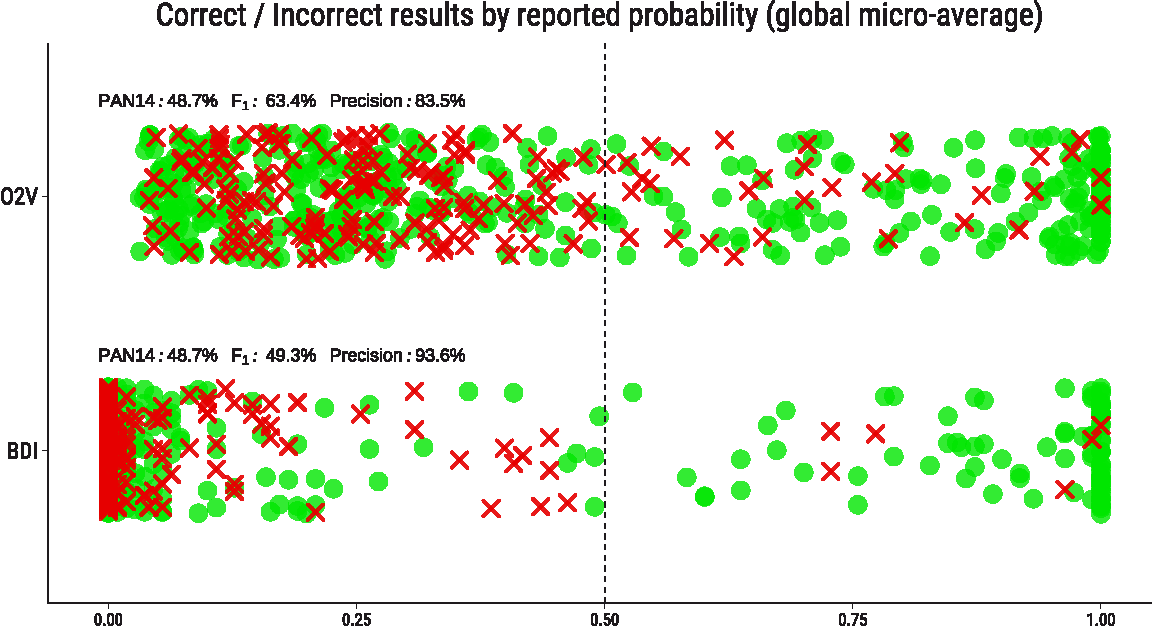
\includegraphics[width=\linewidth]{images/bdi_o2v-crop.pdf}
    \caption{A comparison of the correct and incorrect results by reported probability for BDI
        (manual shifter, 2,3,4,5-grams, minmax) vs Order2Verifer (fitted shifter, 2,3,4,5-grams,
        minmax) on the full PAN 2014 set. Performance metrics are global micro-averages, $n=746$.}
    \label{fig:bdi_o2v}
\end{figure*}


The BDI classifier was compared head-to-head with the updated Kestemont \texttt{Order2Verifier} on
the full PAN 2014 evaluation corpus, which is a challenging set of varied authorial styles across
four languages.%
%
\footnote{ There is a small inconsistency that I was unable to resolve---the only copy of the
    verification problems I could find were archived in the Kestemont repository, but they are
    apparently missing 50 of the `Dutch Reviews' evaluation problems, so there are a total of 746,
    versus 796 reported in the PAN 2014 wrapup report. }
%
Additionally, both verifiers were evaluated below using the PAN 2021 problems, since that competition
included some deep-learning approaches, discussed further below. For this evaluation I used
character $n$-grams, since that feature universe is a generally reliable and uncontroversial choice
for modern stylometric work. There may be feature universes that perform better, or features that
work better for a specific task, but character $n$-grams are `solid if boring'. Likewise, the
$n$-gram frequencies are $z$-scaled (based only on the training variances) since this is the
standard approach. I tested two $n$-gram configurations, 2,3,4-grams and 2,3,4,5-grams, 10,000 max
features, with fitted and manual score shifting. For the \texttt{Order2Verifier} bootstrapping was
performed at 50\% (5000 random features per bootstrap iteration) since that is the configuration
used in \cite{kestemont_caesar}; for BDI, bootstrapping was performed at 33\%. Finally, for the
distance metric used to determine `closeness' at each step I tested the cosine distance (the most
traditional choice) and the minmax (Ružička) metric promoted by Kestemont et al. in their original
paper. Consistent with those results, the minmax metric appears generally superior (see Table
\ref{tab:micro}). The fully reproducible testing code is available in the supplementary repository
\cite{nagy_bdi_2024}. Several metrics are reported, some of which (C@1, F$_{0.5u}$) are rare
outside the PAN competitions, along with the overall evaluation scores for PAN 2014 (AUC$\times$C@1)
and PAN 2021 (mean of the five balanced measures).

\subsection{Results vs PAN 2014}

The format of the PAN 2014 problems makes it straightforward to apply the BDI and GI verifiers and
directly compare the results. As can be seen from Table \ref{tab:micro}, the performance of the BDI
classifier is consistently strong, with only a small boost in PAN score resulting from fitting the
score shifter. When evaluated as a global micro-average (as done in the competition), the `best' BDI
verifier outperformed both updated Kestemont GI and the winning PAN 2014 entrant. It must be noted,
however, that the individual corpus results are not dominated by either verifier but vary
considerably according to evaluation strategy and corpus. The strength of the BDI classifiers,
however, is twofold: first, they do not really require any training corpus, and second, the BDI
approach is high precision (it yields very few false positives), making it a conservative verifier
whose positive results are reliable (at the cost of more false negatives). This can be seen clearly
in Figure \ref{fig:bdi_o2v} in which the best performing GI classifier is compared to a manually
fitted BDI classifier (results between 11\% and 89\% are left unanswered) using the same features
and metrics. This is not the best performing BDI verifier: it was chosen because these verifiers
have an almost identical overall PAN14 score but quite different detailed characteristics. The
results for each subcorpus are broken down in more detail in Tables \ref{tab:bdi} \& \ref{tab:o2v}.
In those tables, the respective results for the \textit{en\_novels} set are of particular interest.
This sub-corpus was extremely challenging, causing problems for all entrants due to the shared-genre
nature of Lovecraftian horror and the unifying force of its pervasive style (explained in more
detail in \cite[882]{pan_2014}). BDI underperformed here according to the PAN metrics, but did so
conservatively, with a perfect precision score of 1.0.

\subsection{Testing vs PAN 2021}

Since the state of the art in authorship verification is now exploring the possibilities offered by
deep learning, the BDI verifier (and the \texttt{Order2Verifier}) were also evaluated using the data
from the PAN 2020--2021 shared task. The final evaluation report from that task is available in
\cite{kestemont2021overview}. The 2020--21 tasks used English-language fan-fiction, which is
available in vast amounts. Although the huge amount of training data and the limitation to English
makes the problems somewhat less interesting, it is interesting to know how much we `lose' by using
simple machine learning approaches that can be widely applied as compared to cutting-edge techniques
applied to best-case scenarios. The large amount of training data (the \textbf{large} training set
contained 176,000 total text pairs, and even these were synthetically augmented by some teams!), as
well as the more recent date, meant that the results here were dominated by complex deep learning
models, with the winning entry being an extremely impressive siamese network using four
subcomponents \cite{boenninghoff:2021}. It is not possible to provide a strict `apples to apples'
comparison, since the entrants were required to assess each problem as an atomic pairwise
determination (were these two texts written by the same author). For the Imposters methods in
general, at least one sample from the candidate author is required, and a pool of imposters is used
at each step. However, the evaluation was done as fairly as possible. Although the BDI and GI
verifiers are not `trained' per-se, both the score shifting parameters for the fitted shifters as
well as the variances used in $z$-scaling were derived from a subset of the \textbf{small} training
corpus. This is in spirit with the real PAN competition where the final evaluation dataset was fully
blinded, unlike in previous years. The amount of training data employed was very small, using just
4256 texts from the `small' training set, which contained 106,000 texts. The final evaluation used
texts from the 2021 evaluation set (19999 pairs) which contained no texts from authors in the
training sets. To fairly assess AUC, a roughly even split of positive and negative determinations
are required. In addition, since the 2021 shared task was focused on previously-unseen authors,
unseen authors were included as noise in both the comparison set (candidate profiles) and the
evaluation set (verification problems). The evaluation set that was eventually used contained 10,152
problems, and was broken down as follows:
\begin{itemize}
    \item 5076 problems from authors with at least one other text, tested against the true label;
    \item 2538 problems from authors with at least one other text, tested against a randomly chosen
          false label;
    \item 2538 problems from unseen authors, tested against a random false label.
\end{itemize}
The candidate/comparison set is composed as follows:
\begin{itemize}
    \item 1692 authors who are never seen again, as noise;
    \item 7451 authors with one comparison sample (who might appear against a true or false label);
    \item 905 authors with 5 comparison samples;
    \item 94 with 11;
    \item 7 with 19;
    \item 3 with 29.
\end{itemize}
As can be seen, the large majority of authors have only one comparison candidate. The unnatural
distribution of counts for texts per author is an artifact of the PAN data, and is presumably
related to the corpus compilation process. The evaluation process used all of the evaluation texts
by authors with two or more total samples, but the bulk of the singleton texts were not used. The full
evaluation process is available as commented Jupyter notebooks at the accompanying repository.
\begin{table}
    \caption{Fitting Results: PAN 2021 (small training corpus), 1000 problems}
    \label{tab:p20fit}
    % \par\medskip
    \raggedright
    \begin{adjustbox}{max width=\textwidth}
        \begin{tabular}{lllrrrrrrrrrr}
            \toprule
                                                      &                                     &         & U_{count} & U_{low} & U_{hi} & Prec           & AUC            & C@1            & F_{0.5u}        & F_1            & Brier          & PAN21        \\
            Verifier                                  & Vectorizer                          & Shifter &           &         &        &                &                &                &                &                &                &                \\
            \midrule
            \multirow[c]{4}{*}{BDI, Cosine }          & \multirow[c]{2}{*}{ 2,3,4,5-grams } & fitted  & 94        & 0.089   & 0.661  & 0.960          & 0.942          & 0.911          & 0.902          & 0.917          & 0.910          & 0.917          \\
                                                      &                                     & manual  & 131       & 0.110   & 0.890  & 0.979          & 0.939          & 0.909          & 0.893          & 0.918          & 0.906          & 0.913          \\
                                                      & \multirow[c]{2}{*}{ 2,3,4-grams }   & fitted  & 95        & 0.205   & 0.741  & 0.970          & 0.947          & 0.920          & \textbf{0.909} & 0.923          & 0.914          & 0.923          \\
                                                      &                                     & manual  & 146       & 0.110   & 0.890  & 0.979          & 0.944          & 0.916          & 0.892          & 0.931          & 0.909          & 0.918          \\
            \multirow[c]{4}{*}{BDI, Minmax }          & \multirow[c]{2}{*}{ 2,3,4,5-grams } & fitted  & 101       & 0.169   & 0.822  & 0.977          & 0.941          & 0.913          & 0.906          & 0.916          & 0.908          & 0.917          \\
                                                      &                                     & manual  & 136       & 0.110   & 0.890  & 0.979          & 0.937          & 0.907          & 0.891          & 0.918          & 0.906          & 0.912          \\
                                                      & \multirow[c]{2}{*}{ 2,3,4-grams }   & fitted  & 120       & 0.125   & 0.724  & 0.973          & \textbf{0.951} & \textbf{0.924} & 0.905          & 0.935          & \textbf{0.918} & \textbf{0.927} \\
                                                      &                                     & manual  & 149       & 0.110   & 0.890  & 0.979          & 0.948          & 0.919          & 0.894          & 0.936          & 0.914          & 0.922          \\
            \multirow[c]{4}{*}{Kestemont GI, Cosine } & \multirow[c]{2}{*}{ 2,3,4,5-grams } & fitted  & 119       & 0.312   & 0.777  & 0.966          & 0.944          & 0.913          & 0.898          & 0.924          & 0.909          & 0.918          \\
                                                      &                                     & manual  & 328       & 0.110   & 0.890  & 0.981          & 0.920          & 0.857          & 0.830          & 0.964          & 0.875          & 0.889          \\
                                                      & \multirow[c]{2}{*}{ 2,3,4-grams }   & fitted  & 130       & 0.312   & 0.741  & 0.966          & 0.947          & 0.921          & 0.898          & 0.936          & 0.911          & 0.923          \\
                                                      &                                     & manual  & 346       & 0.110   & 0.890  & 0.981          & 0.916          & 0.847          & 0.819          & 0.966          & 0.873          & 0.884          \\
            \multirow[c]{4}{*}{Kestemont GI, Minmax } & \multirow[c]{2}{*}{ 2,3,4,5-grams } & fitted  & 104       & 0.393   & 0.786  & 0.973          & 0.943          & 0.915          & 0.906          & 0.921          & 0.912          & 0.920          \\
                                                      &                                     & manual  & 328       & 0.110   & 0.890  & 0.984          & 0.919          & 0.857          & 0.831          & 0.965          & 0.875          & 0.889          \\
                                                      & \multirow[c]{2}{*}{ 2,3,4-grams }   & fitted  & 132       & 0.312   & 0.741  & 0.971          & 0.950          & \textbf{0.924} & 0.902          & 0.940          & 0.914          & 0.926          \\
                                                      &                                     & manual  & 338       & 0.110   & 0.890  & \textbf{0.984} & 0.924          & 0.858          & 0.831          & \textbf{0.972} & 0.876          & 0.892          \\
            \bottomrule
        \end{tabular}
    \end{adjustbox}
\end{table}

\begin{table}
    \caption{Evaluation Results: PAN 2021, 10,152 test problems}
    \label{tab:p20eval}
    % \par\medskip
    \raggedright
    \begin{adjustbox}{max width=\textwidth}
        \begin{tabular}{llrrrrrrrrrr}
            \toprule
                                                      &                  & U_{count} & U_{low} & U_{hi} & Prec           & AUC            & C@1            & F_{0.5u}        & F_1            & Brier          & PAN21        \\
            Verifier                                  & Shifter          &           &         &        &                &                &                &                &                &                &                \\
            \midrule
            \multirow[c]{3}{*}{BDI, Minmax }          & fitted           & 1326      & 0.125   & 0.724  & 0.975          & 0.922          & 0.881          & 0.872          & 0.882          & 0.885          & 0.889^{*}      \\
                                                      & fitted (optimal) & 1128      & 0.053   & 0.393  & 0.943          & \textbf{0.924} & \textbf{0.889} & \textbf{0.876} & 0.896          & \textbf{0.892} & \textbf{0.896} \\
                                                      & manual           & 1815      & 0.110   & 0.890  & 0.984          & 0.918          & 0.870          & 0.843          & 0.877          & 0.878          & 0.877          \\
            \\
            \multirow[c]{3}{*}{Kestemont GI, Minmax } & fitted           & 1385      & 0.312   & 0.741  & 0.974          & 0.923          & 0.874          & 0.865          & 0.874          & 0.888          & 0.885          \\
                                                      & fitted (optimal) & 1433      & 0.196   & 0.527  & 0.940          & \textbf{0.924} & 0.883          & 0.863          & 0.898          & 0.891          & 0.892          \\
                                                      & manual           & 3578      & 0.110   & 0.890  & \textbf{0.987} & 0.892          & 0.820          & 0.774          & \textbf{0.931} & 0.860          & 0.855          \\

            \\
            BDI, Minmax , unranked                    & fitted           & 1469      & 0.125   & 0.724  & 0.982          & 0.915          & 0.859          & 0.847          & 0.848          & 0.868          & 0.867          \\
            Kestemont GI, Minmax , unranked           & fitted           & 940       & 0.312   & 0.741  & 0.982          & 0.917          & 0.841          & 0.855          & 0.809          & 0.858          & 0.856          \\
            \bottomrule
        \end{tabular}
    \end{adjustbox}
\end{table}

Overall, the best performers in training were fitted versions of the 2,3,4-gram Kestemont GI and BDI
verifiers, once again with the minmax metric. The full results can be seen in Table
\ref{tab:p20fit}. Since the bootstrapping process was extremely time consuming on the full
evaluation set, only the 2,3,4-gram vectorizer was used. The best performing BDI verifier posted a
final overall score of 0.889, using the PAN 2021 metric (the mean of several accuracy measures,
calculated using the official evaluation code). This would place it near the bottom of the four
``strong runner ups'' \cite[7]{kestemont2021overview}, still comfortably outperforming the
machine-learning benchmarks and 5 human teams. It seems reasonable to assume that a more
sophisticated feature vector, such as the one used in weerasinghe21 \cite{weerasinghe2021feature},
would improve the performance of both Order2Verifier and BDI. By comparison, the final score for
boenninghoff21 was 0.9545. Once again, it is clear from Tables \ref{tab:p20fit} and
\ref{tab:p20eval} that the fitting is nice to have in terms of the overall PAN21 score (which uses
several balanced accuracy measures), but in fact reduces raw precision, which is relevant where
research problems require the smallest chance of false positives.

As further exploration, some differential / ablation results are included in Table
\ref{tab:p20eval}. The results under the shifter method `fitted (optimal)' calculate the optimal
post-hoc \texttt{p1} and \texttt{p2} (as discussed above) based on the results from the evaluation
itself---in other words it shows the advantage if the training regime were to perfectly represent
the probability distribution of the true problems. As can be seen, this is quite minor (an overall
score of 0.896 vs 0.889), which is encouraging. However, the relatively strong performance of the
manual shifter with the BDI verifier, as well as its higher precision, seems to suggest that the
small increase in some of the measures does not warrant the methodological uncertainty (in terms of
representativeness and bias) added by the fitting process in general. Additionally, it can be seen
that the score shifting optimisation is very sensitive to the evaluation measure, incurring quite a
large precision penalty---not a component of the target metric---in order to improve the overall
score. Finally, the new addition of `ranking' was evaluated by ablation. As in the PAN 2014 results
(Table \ref{tab:micro}, PAN14-U), the ranking regularisation appears to offer a small but consistent
benefit to AUC and F-measures, which is impressive considering how few of the authors (about 10\%)
had more than one comparison sample. The unranked verifiers, however, showed even higher precision
which may need to be considered for some applications.

\section{Showcase}\label{sec:showcase}

This section refers to two verification studies in which BDI has been applied, one of which is, at
the time of writing, still in press. These figures are not full summaries of the research, but
simply illustrate some of the features of the BDI method that I believe to be useful. As mentioned
above, the output of the BDI algorithm is a distribution of distances, not a summary statistic.
These examples attempt to show that examining the full distribution conveys extra information and
can improve our intuition and confidence in the analysis.

\begin{figure*}
    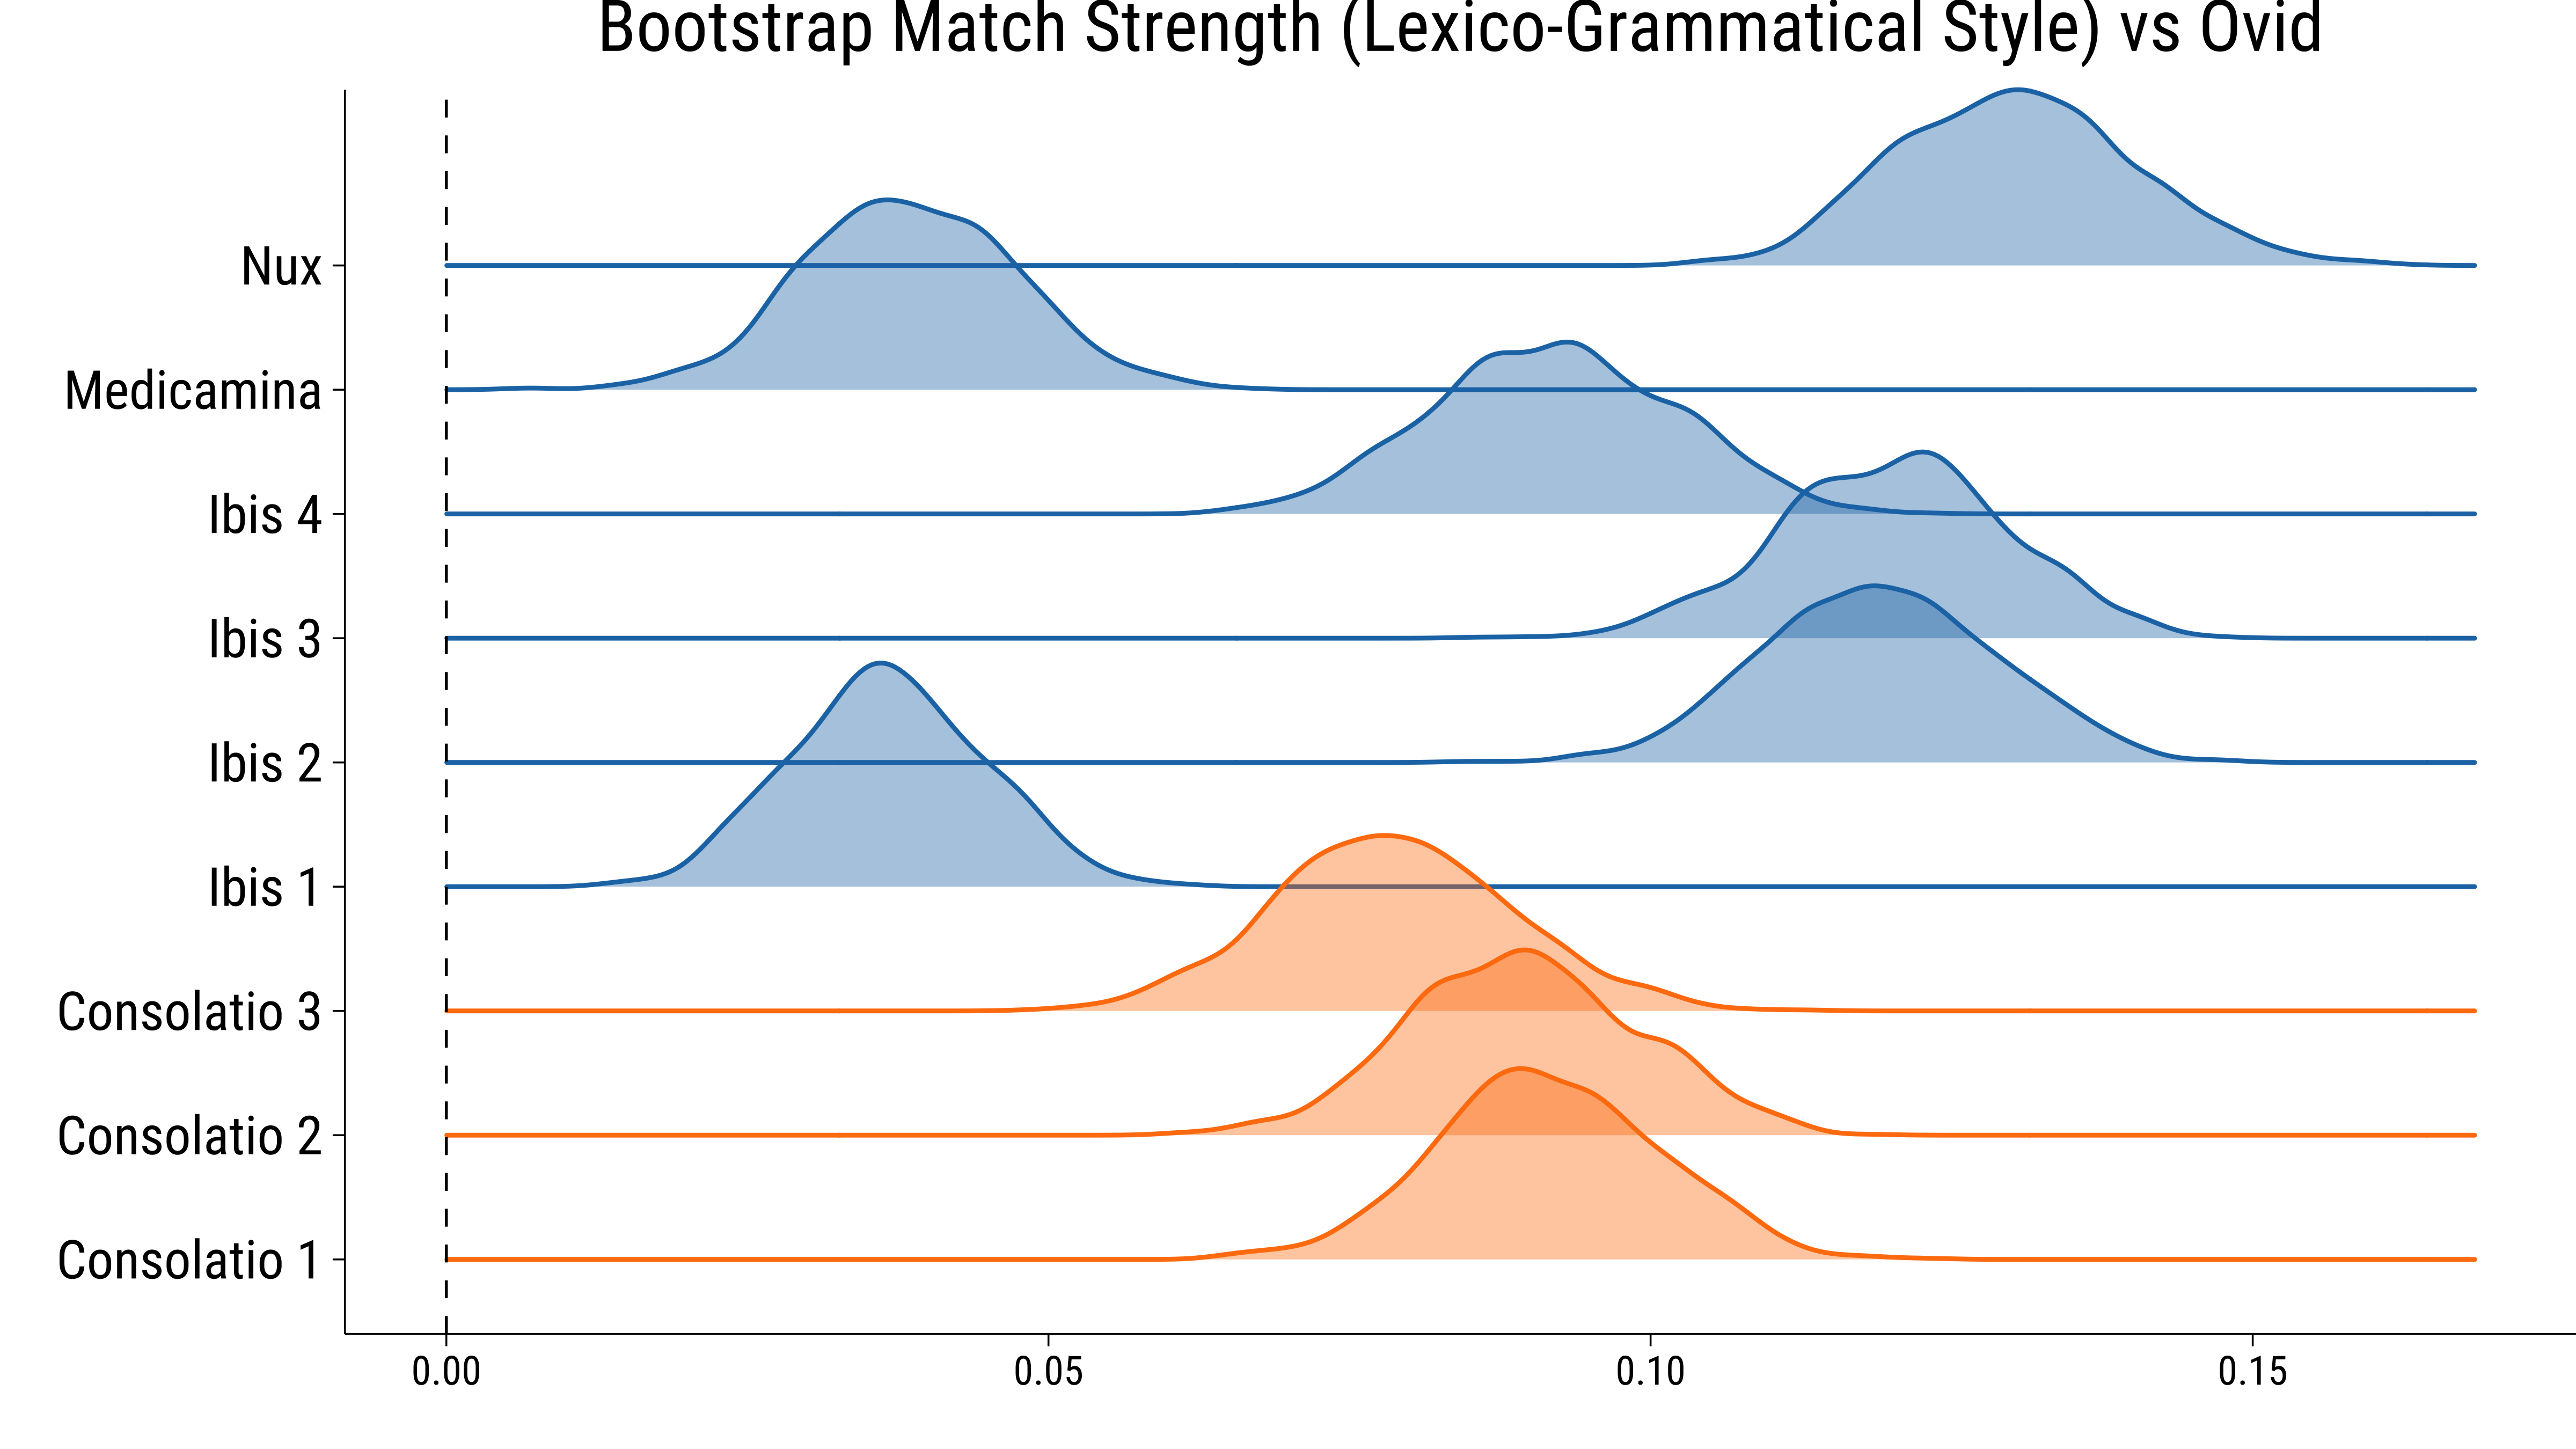
\includegraphics[width=\linewidth]{images/bootstrap_lexical_paper.png}
    \caption{A BDI comparison of several works attributed to Ovid using
        lexico-grammatical features (character $n$-grams). The \emph{Consolatio Ad
            Liviam} is now considered to be a first-century imitation.}
    \label{fig:nux_lex}
\end{figure*}

\begin{figure*}
    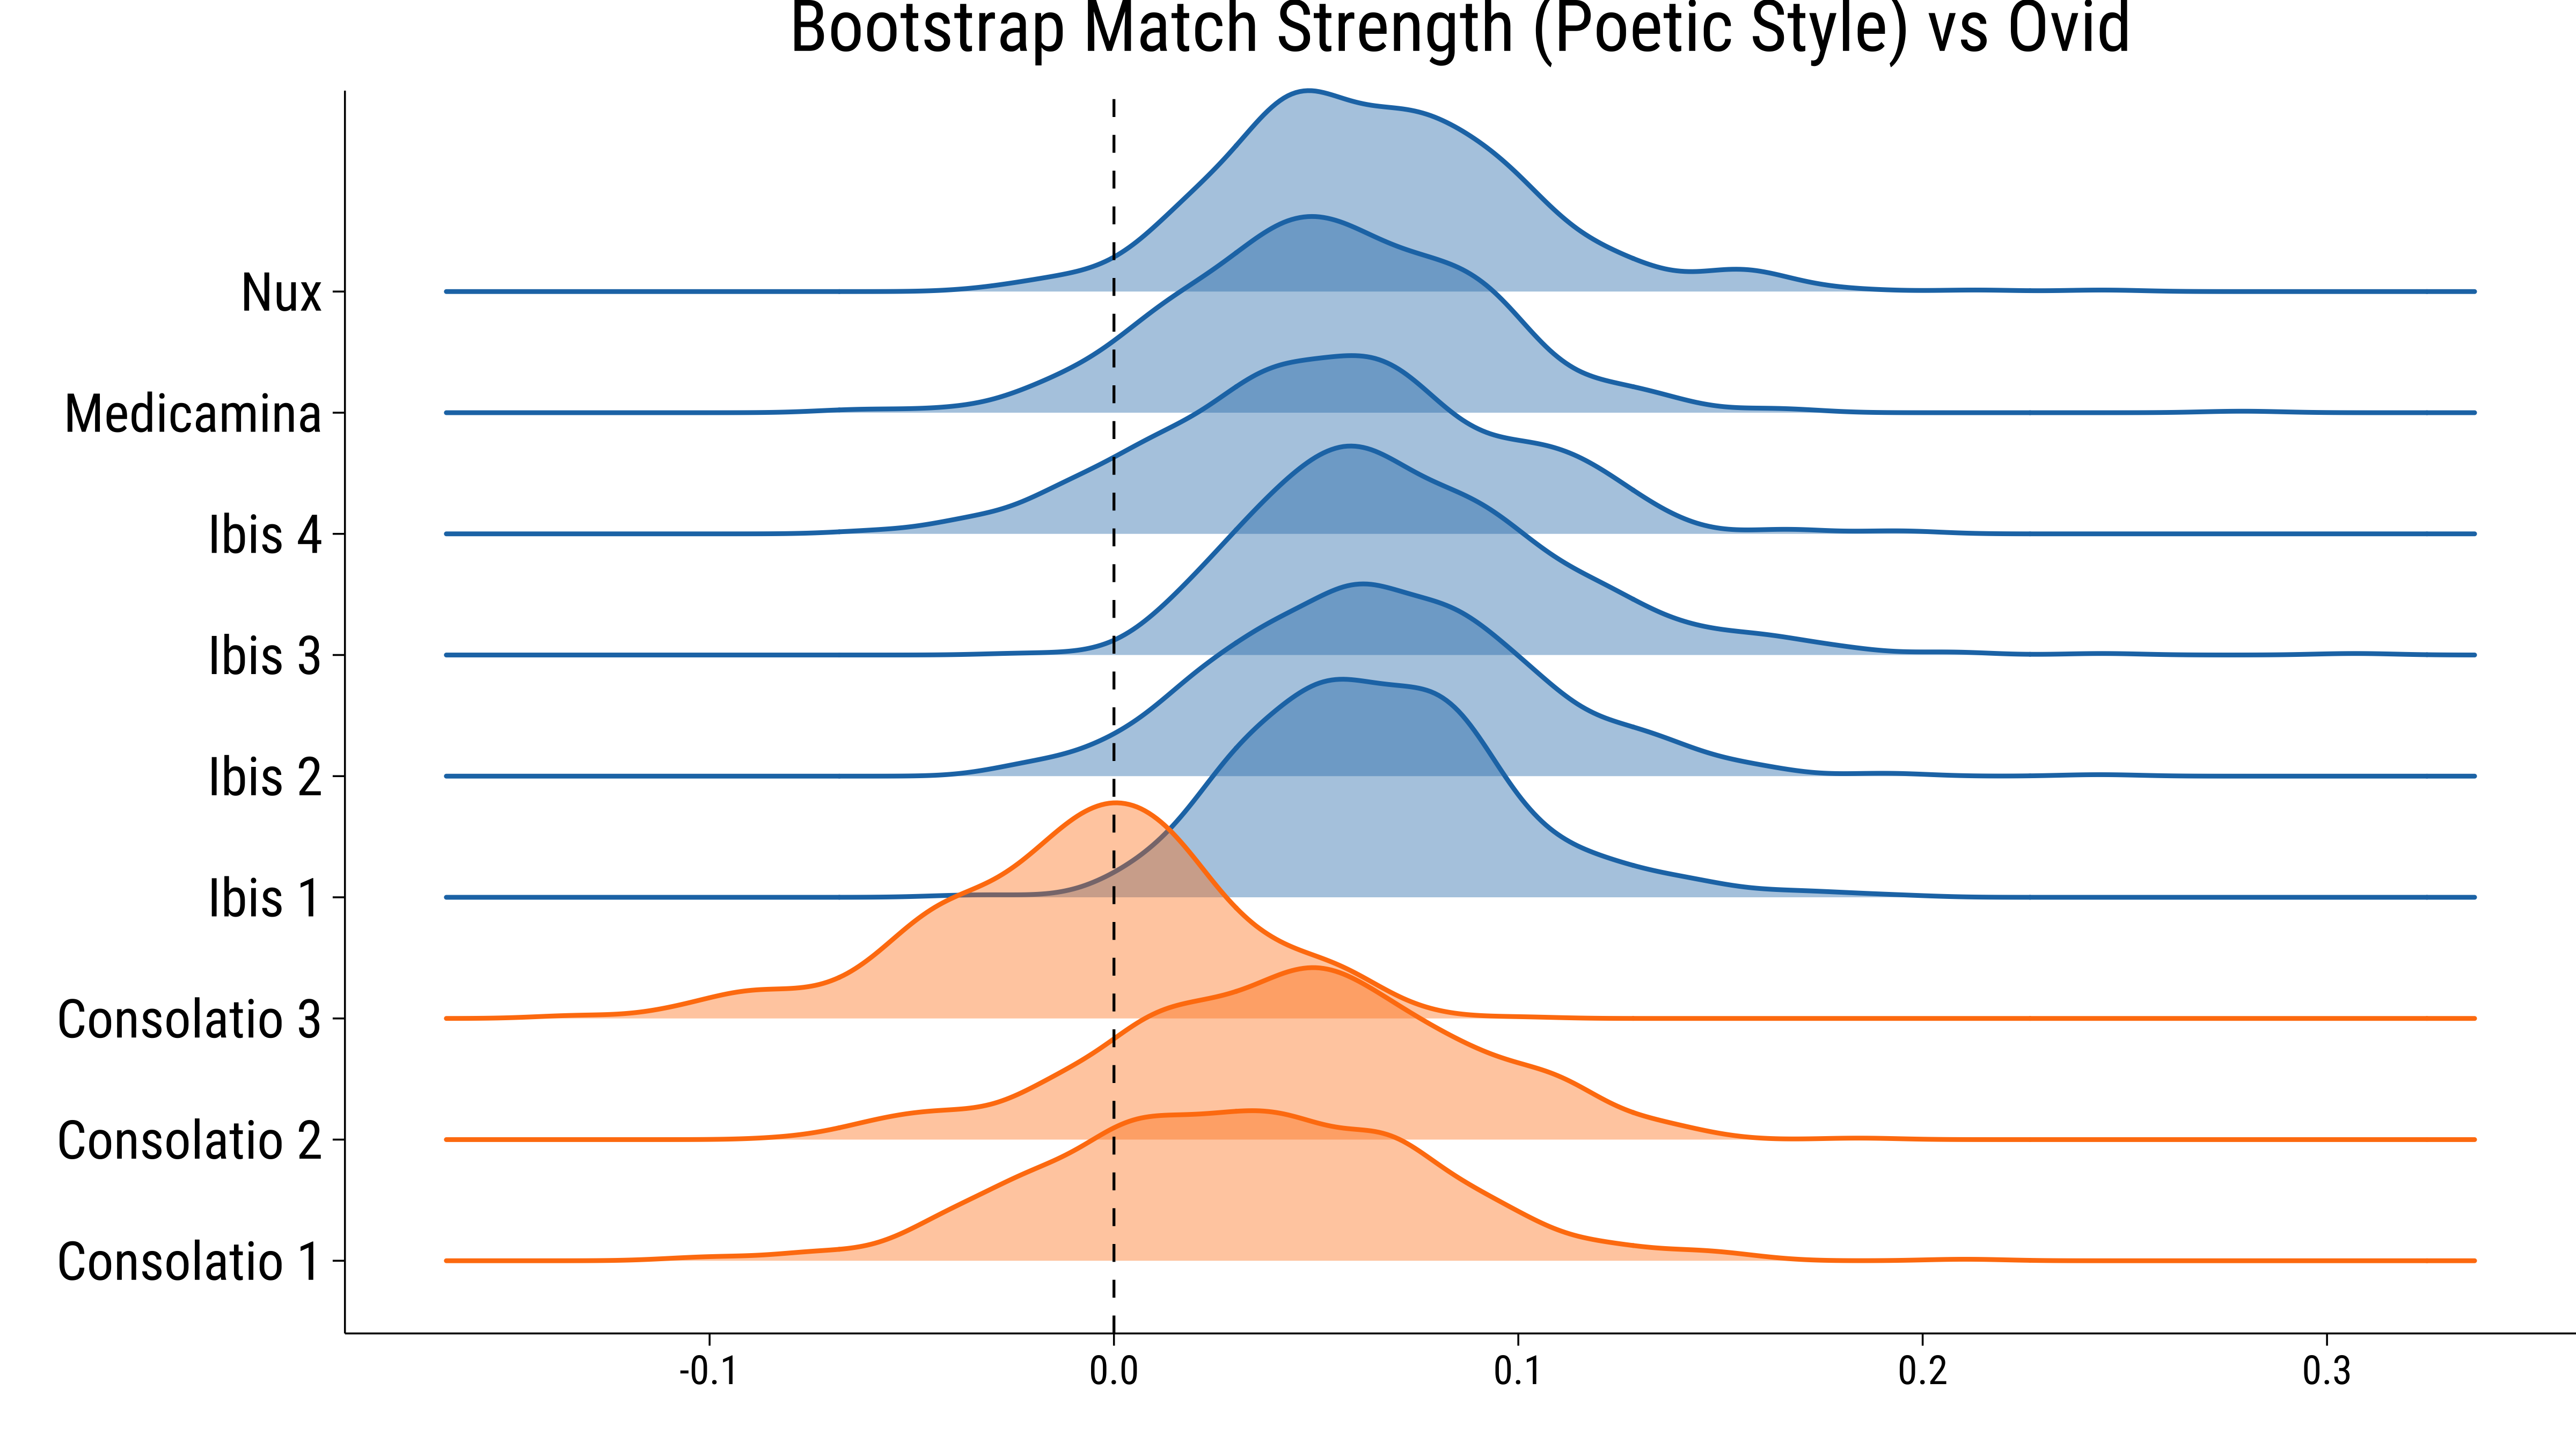
\includegraphics[width=\linewidth]{images/bootstrap_poetics_paper.png}
    \caption{A BDI comparison of the same works attributed to Ovid, examining
        poetic/metrical features of Latin dactylic elegy instead of lexical
        features.}
    \label{fig:nux_poet}
\end{figure*}

Figures \ref{fig:nux_lex} \& \ref{fig:nux_poet} are from an analysis of several poems attributed to
Ovid. The aim here was to provide evidence for the genuineness of the \emph{Nux}, but of more
interest in this context is the analysis of the \emph{Consolatio ad Liviam}. The \emph{Consolatio}
was once considered to be a genuine work of Ovid, but is now accepted by most scholars to be a
first-century imitation. By using BDI we attempted to show that metrical technique was a powerful
enough stylistic feature to disambiguate even deliberate imitation from genuine works. In Figure
\ref{fig:nux_lex}, we see the value of visualising distributions where all of the distances are
positive (closer to the candidate author than an imposter), which would be summarised as a
`probability' of 1.0. This figure measures similarity in terms of lexico-grammatical features,
operationalized as character $n$-grams. In fact, as can be seen, although the chunks from the
\emph{Consolatio} are much more like Ovid than they are like any of the distractor poets, they are
\emph{not as much like} Ovid as most of the candidate comparison works. This kind of comparability
between strong matches is very difficult with the standard GI approach. However, in Figure
\ref{fig:nux_poet}, which measures metrical features, the difference is clear---the sections from
the \emph{Consolatio} are centered around 0 (or near enough) as compared to the other works where at
least 90\% of the distribution mass is above 0, supporting a positive attribution. This result
suggests that the \emph{Consolatio} is not Ovidian, but also that it is not a good stylistic match
for any of the distractor poets (Tibullus, Propertius, and Catullan elegy). This is consistent with
the  current (weak) consensus that the \textit{Consolatio} is a late first-century imitation by an
unknown.

\begin{figure*}
    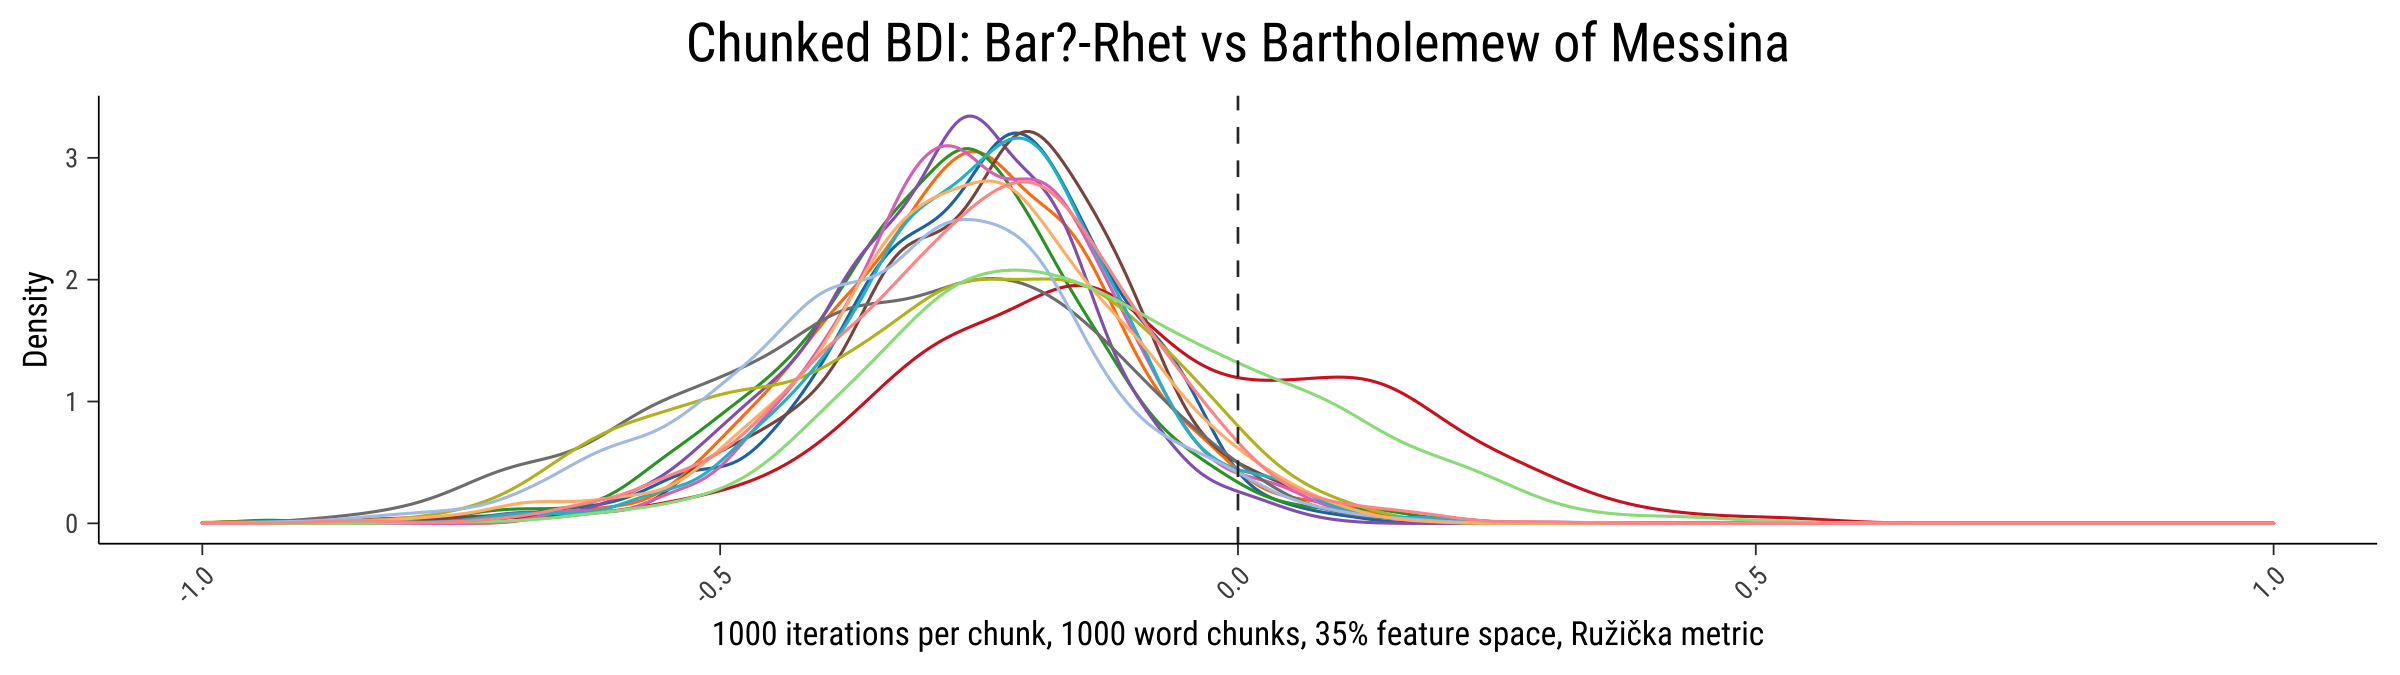
\includegraphics[width=\linewidth]{images/bdi_bar_paper.png}
    \caption{A BDI comparison of use of Latin function words to match a
        translation of Aristotle's \emph{Rhetoric} to Bartholemew of Messina. Each
        distribution is the full BDI run for one chunk of the work.}
    \label{fig:trans_bar}
\end{figure*}

\begin{figure*}
    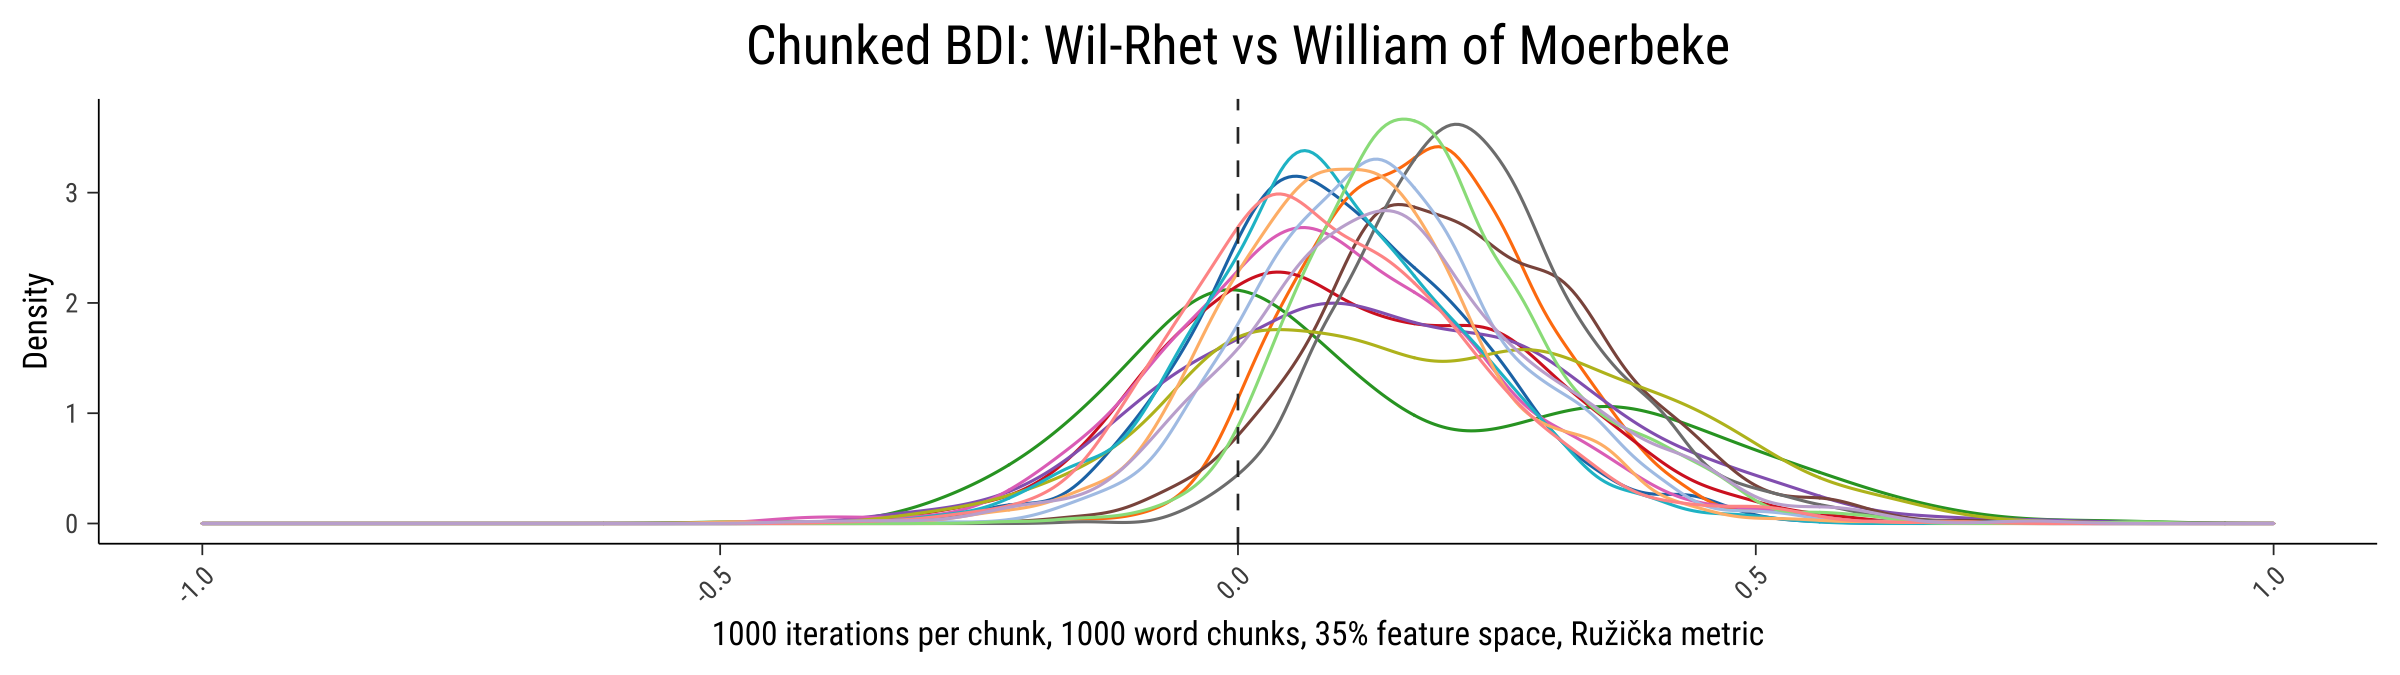
\includegraphics[width=\linewidth]{images/bdi_wil_paper.png}
    \caption{A BDI comparison of use of Latin function words to match a
        translation of Aristotle's \emph{Rhetoric} to William of Moerbeke. Each
        distribution is the full BDI run for one chunk of the work.}
    \label{fig:trans_wil}
\end{figure*}

Figures \ref{fig:trans_bar} \& \ref{fig:trans_wil} are from an analysis of translator style,
examining medieval translations from Greek to Latin. Translator style (as opposed to authorial
style) offers a unique set of challenges, covered in much more detail in the full paper
\cite{Beullens_Haverals_Nagy_2024}. In this study, a small set of function words was used, in
accordance with the well-known theory that closed-class words are used more unconsciously, and thus
are more indicative of individual preferences than nouns, verbs, and adjectives (which are highly
affected by genre and topic). Overall, this was found to be an effective approach. Here, however, I
note two more useful properties of the BDI method. The first is that by splitting the work into
smaller chunks, and visualising the distribution for each chunk we are able to see the degree of
stylistic variation in a single translator. It is also clear from Figure \ref{fig:trans_bar} that
some passages are less `stylistically clear', showing much more pronounced spread---this can be
interpreted as greater sensitivity to the individual feature subsets. Overall, Figure
\ref{fig:trans_bar} is centred around a negative value, indicating that it is significantly more
similar to one of the imposter translators than to Bartholemew. In Figure \ref{fig:trans_wil}, we
performed the same process for a different text that is a translation of the same work (Aristotle's
\emph{Rhetoric}) generally accepted to be by William of Moerbeke. In the latter case we see the
expected result---almost all of the chunks are fairly strongly centred around a positive value. The
strength of the match is not as clear as in the Ovidian figures, but this is perhaps to be expected,
since the amount of style that a translator brings to a work can be reasonably assumed to be less
than that brought by an author (this is a well studied field; see for example
\cite{rybicki2012great} with references).

\section{Future Work}

As can be seen from Figure \ref{fig:bdi_o2v}, predictions from the BDI classifier (after shifting)
cluster strongly at the extremes, with most mis-predictions being high-confidence false negatives.
The Kestemont GI classifier shows the most mis-predictions in the central band (near 0.5), which is
intuitive if the outputs are interpreted as probabilities. The current link function from the BDI
distributions to a `probability' in $[0,1]$ is a fairly simple idea, and can almost certainly be
improved to produce a smoother and more statistically informed distribution across the output range
(perhaps logistic regression, or even empirical distributional statistics). This is left for future
work.

\section{Conclusions}

The most common goal in authorship verification work is to positively attribute works to authors. In
this context, although balanced accuracy is not unimportant, precision (fewer false positives) is
often more important than recall. The balanced metrics used for the PAN 2014 / 2021 authorship
verification competitions balance overall AUC (false positives and false negatives) with the ability
for a classifier to degrade gracefully when the result is unclear. In general, this is a useful
innovation, particularly in comparison to standard machine-learning classifiers which are obliged to
assign each problem to a discrete class (even if the true author is not one of the available
answers). While the widely-used General Imposters method still performs extremely well, it seems
wasteful to discard the detailed distance information that is calculated in any case during the
bootstrap / voting process.

BDI attempts to address these issues by outputting a full distance distribution which can be
manually inspected. As demonstrated in Section \ref{sec:showcase}, this can be very useful when
comparing results that are all strong matches. When operating as a summary verifier, BDI tends to be
conservative in its positive attributions, particularly when applied to very difficult problem sets
like the PAN2014 \textit{en\_novels}. In terms of raw performance, the BDI verifier appears slightly
stronger than the improved Kestemont GI according to the PAN metrics for both the 2014 and 2021
problems, while also offering superior interpretability. The advantage of the BDI verifier is even
clearer when score shifting is not used. Overall, the BDI approach seems to be a strong choice,
especially where training data is limited and/or reliable positive results are more important than
balanced performance metrics. 

\section{Availability of Data and Code}\label{sec:data}

The preprint may be found at \url{https://github.com/bnagy/bdi-paper}. All code and data is
available under CC-BY, except where restricted by upstream licenses. The code repository includes
full reproduction data and code for the evaluation, as well as various supplemental figures and
explanations.

\FloatBarrier

%%
%% The acknowledgments section is defined using the "acknowledgments" environment
%% (and NOT an unnumbered section). This ensures the proper
%% identification of the section in the article metadata, and the
%% consistent spelling of the heading.
\begin{acknowledgments}
    This work was supported by project 2020/39/O/HS2/02931, funded by Poland's National Science Centre
\end{acknowledgments}

%%
%% Define the bibliography file to be used
%\bibliography{bdi_refs}
\printbibliography
%%
%% If your work has an appendix, this is the place to put it.
\appendix
\onecolumn

\end{document}

%%
%% End of file